\section{Approach}

\subsection{Baseline method}
We take an intuitive approach as our baseline, which we call the 
most frequent noun.act.
Given an action concept \emph{subject verb object} where \emph{subject} 
and \emph{object} are both concept, e.g., \emph{country} invade \emph{country}.
$S_{verb}$ is the set of verb's synonyms in WordNet. 
Since an action triple doesn't provide adequate information for verb sense 
disambiguation, we take all synsets as verb's synonyms. $D_{verb}$ is 
the the set of words derivable from the verbs in $S_{verb}$,
from which we choose those whose semantic field (or lexical file name) 
in WordNet is noun.act. \KZ{These are nouns that has the semantics of an action,
such as XXX and YYY.} The first-K nouns with highest frequency
 counts are taken as our candidates. If one noun belongs to several 
synsets annotated as noun.act, the frequencies are combined to represent
the frequency counts of that noun.
\begin{align}
    S_{verb} & = \{{ v \in S_i | S_i \ synset \ of \ verb}\} \\
    NA_{verb} & = \{{ NA_i \ d.r.w.  \ of \ s_i | s_i \in S_{verb}}\} \\
    S_{noun} & = \{{ n \in S_i | S_i \ synset \ of \ noun, noun \in NA_{verb}}\}
\end{align}


\subsection{Retrieval based method}

Under the assumption that nouns in news titles are likely to be good candidates
for abstraction of action instances in the news bodies, we use a TF-IDF 
based retrieval method to discover action-noun mappings.

\begin{figure}[!htp]
 \centering
 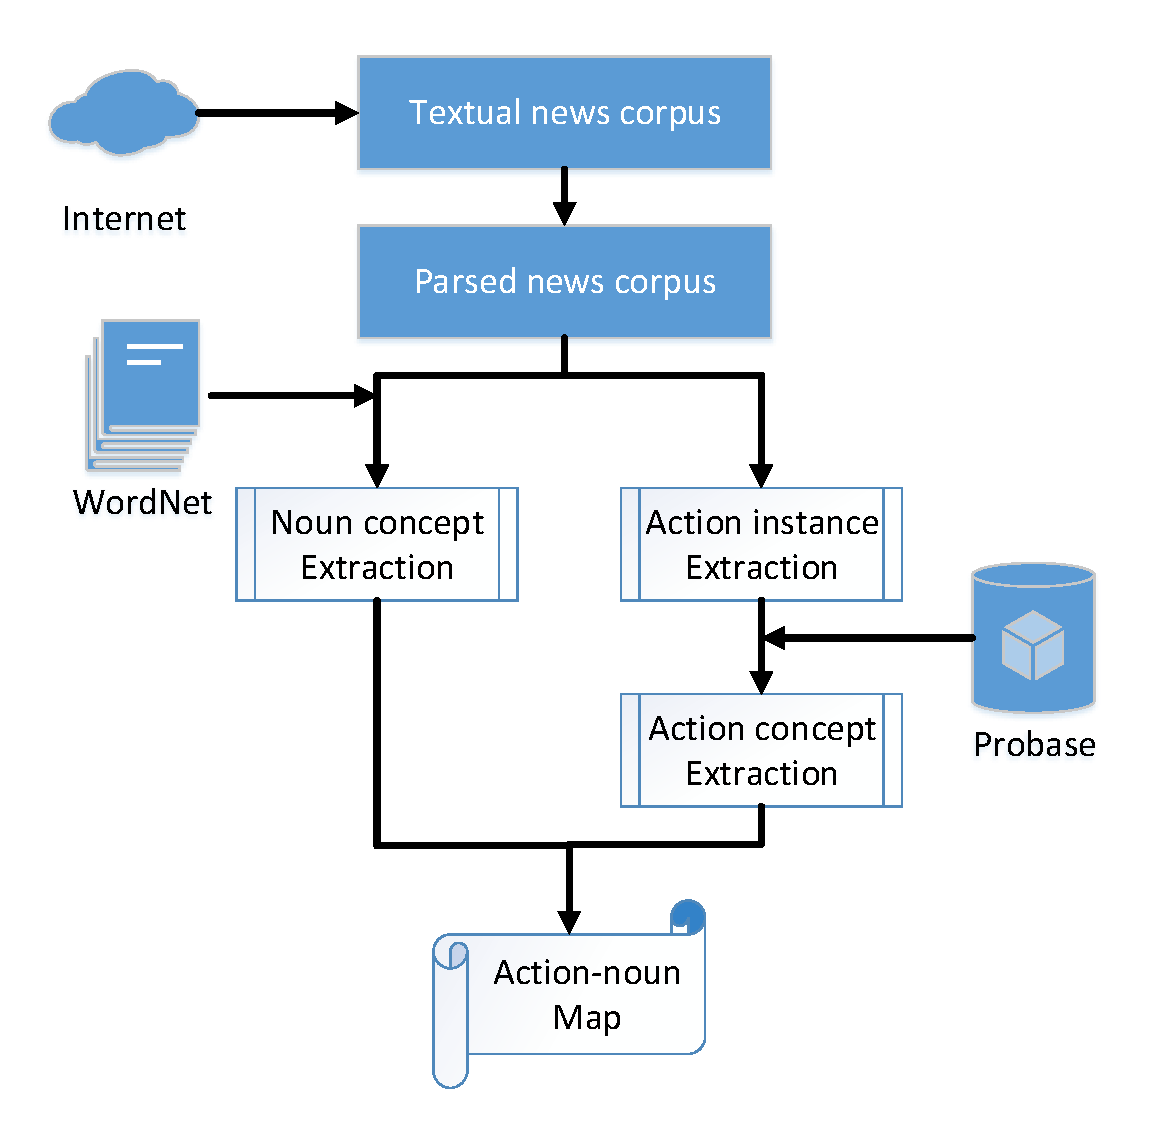
\includegraphics[width=\linewidth]{img/flow.pdf}
 \caption{Work flow}
\end{figure}

We first build our noun dictionary $D$. Here the main sources we use 
are Wordnet, Probase and Wikitionary. 
In wordnet there is a field called lexical info for each token,
such as "noun.act", "noun.state". We can use these information to generate an
initial pool of nouns. At this stage Probase could be used in two ways. 
First it can also be used as a pool generator. 
We can build the noun pool by manually designing
a small set of terms that has desired nouns as hyponyms, such terms include "activity",
"process", "event" etc. Secondly probase can also be used as a filter. We check how
many instances a noun could have and use it as a measurement to decide whether it
is abstract noun or concrete instances. Probase also provides the likelihood of
the hypernym-hyponym relations which we could use too. Wikitionary is an online
dictionary, we found a list of top 10000 popular English word there, hoping to
solve the problem that some words in Wordnet or Probase are too obsolete.
Overall we have 4 different methods to generate the dictionary:
\begin{enumerate}
\item Use top 10000 English word as initial pool and filter by Probase
\item Use Wordnet noun iterator, combined with lexical info to build the initial pool and filter by Probase
\item Use Probase to generate the initial pool and filter by Probase
\item Use Wordnet noun iterator, combined with lexical info, no filtering
\end{enumerate}


Next we find the distribution of noun concepts in news titles, $f_n(i)$, and the distribution of action instances in news bodies,
denoted as $f_{ac}(i)$
\begin{align*}
    f_n(i) & = \{ j |  i \in t_j \} \\
    f_{ac}(i) &= \{ k | i \in b_k \}
\end{align*}
where $t_i$ and $b_i$ are title and body of $i^{th}$ news, respectively.

Next we use TFIDF to compute the relatedness of nouns to actions.
\begin{equation*}
    freq(n_i, ac_j) = \bigm| \{ k | n_i \in t_k \land ac_j \in b_k \} \bigm|
\end{equation*}
\begin{equation*}
    TF(n_i, ac_j) = \begin{cases} 0 &\mbox{if freq is 0} \\
        1 + log(freq(n_i, ac_j)) &\mbox{otherwise}
    \end{cases}
\end{equation*}


\begin{equation*}
    docfreq(n_i) = \bigm| \{ k | n_i \in t_k \} \bigm|
\end{equation*}


\begin{equation*}
    IDF(n_i) = log(\frac{\text{news corpus size}}{1 + docfreq(n_i)})
\end{equation*}
